\documentclass{standalone}
\pagenumbering{gobble}
\usepackage[utf8]{inputenc}
\usepackage{tikz}
\usetikzlibrary{shapes.geometric, arrows}

\tikzstyle{startstop} = [thick, rectangle, rounded corners, minimum width=3cm, minimum height=1cm,text centered, draw=black]
\tikzstyle{io} = [trapezium, trapezium left angle=70, trapezium right angle=110, minimum width=3cm, minimum height=1cm, text centered, draw=black]
\tikzstyle{process} = [rectangle, minimum width=3cm, minimum height=1cm, text centered, text width=3cm, draw=black]
\tikzstyle{decision} = [diamond, minimum width=3cm, minimum height=1cm, text centered, draw=black]
\tikzstyle{arrow} = [thick,->,>=stealth]

\begin{document}

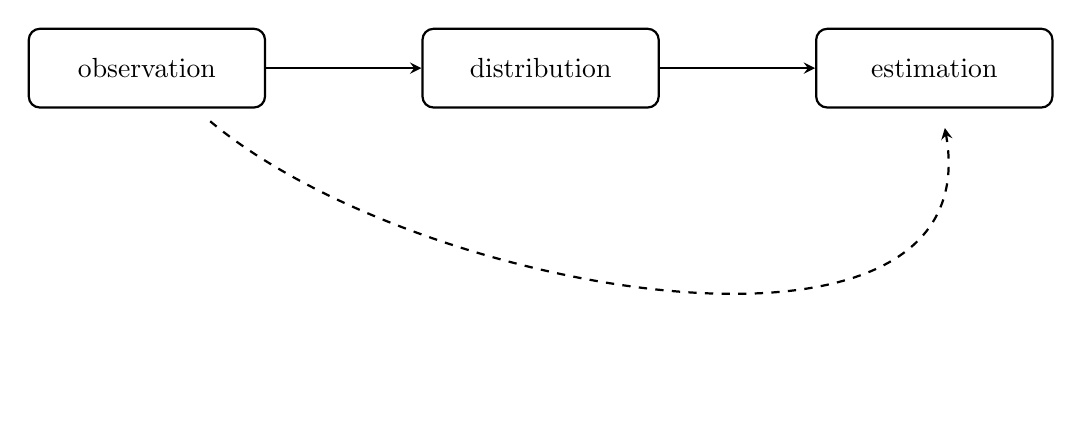
\begin{tikzpicture}[node distance=5cm]

\node (q1) [startstop] {observation};
\node (q2) [startstop, right of=q1] {distribution};
\node (q3) [startstop, right of=q2] {estimation};


\draw [arrow] (q1) -- (q2);
\draw [arrow] (q2) -- (q3);
\draw [arrow, dashed, shorten <= 0.25cm, shorten >= 0.25cm] (q1) to[out=-40,in=-80] (q3);

\end{tikzpicture}

\end{document}